%!TEX root = ../thesis.tex

\chapter{Umsetzung}
\label{chap:coding}
In diesem Kapitel wird auf den Aufbau der Implementierung eingegangen. Anfänglich werden einmalige Vorbereitungsschritte aufgeschlüsselt, hierzu gehört zu einem großen Teil die Kalibrierung der genutzten Kamera in \prettyref{sec:camera} und die Bestimmung der Charakteristika dieser. 

Darauf folgt in \prettyref{sec:board} die Kalibrierung und die Erkennung der Felder des Dartboardes. Es werden verschiedene getestete Ansätze erörtert und ihre Vor- und Nachteile dargestellt.

Anschließend wird die Pipeline im \prettyref{sec:pipeline} allgemein erläutert, um einen Überblick auf die sich wiederholenden Schritte zur Darts Erkennung zu gewähren.

Des Weiteren werden die einzelnen Abschnitte der Pipeline näher beleuchtet und auf die Implementierung und das Vorgehen eingegangen. Dies umfasst von der Segmentierung der Dinge, die nicht zum Dartboard gehören in \prettyref{sec:segmentation}. Bis hin zur konkreten Bestimmung der erzielten Punktzahl in \prettyref{sec:score}. 
\todo{Umsetzung einteilen und implementieren}
\section{Kamera Kalibrierung}
\label{sec:camera}
Um genauere und bessere Daten aus der Kamera ziehen zu können müssen vorher einige Parameter bestimmt werden. Im \prettyref{sec:basics} wurde bereits das Kamera Modell erläutert. 
Zur Bestimmung der erwähnten Parameter. \textquote{Camera calibration is a necessary step in 3D computer vision in order to extract metric information
from 2D images.} \autocite[5]{Zhang2000}

\section{Erkennung des Dartboards}
\label{sec:board}
Stage 1 Board finden:
     mehrere Ansätze
     Blobs des boardes erkennen
     Felder Kanten erkennen
     Board Kalibrieren als Erweiterung der Kamera Kalibrierung
        
        Dartboard Koordinaten bestimmen im Verhältnis zur Kamera.
       Eigentliche Kalibrierung via klicken,
       wie viele Punkte sind nötig
       
\section{Pipeline Überblick}
\label{sec:pipeline}
\begin{figure}
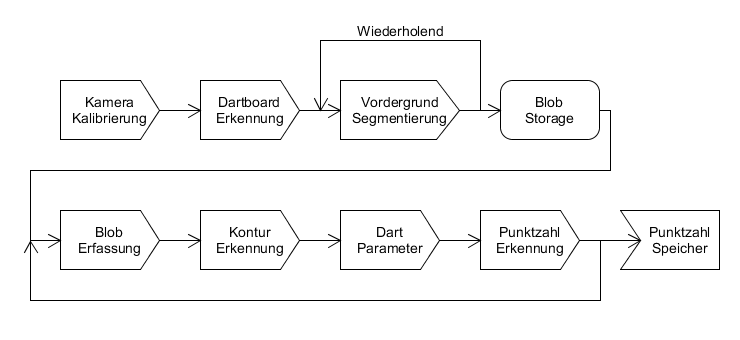
\includegraphics[width=\textwidth]{media/pipeline.png}\\
\caption{\textbf{Übersicht der einzelnen Schritte}}
\label{Fig:pipeline}
\end{figure}

\section{Segmentierung des Vordergrundes}
\label{sec:segmentation}
Stage 3 Vordergrund von Hintergrund trennen
Foreground detection naiver Ansatz und Algorithmen
Parameter Erklärung
Vereinfachung und Annahmen
Aufgetretene Problematik
\section{Verarbeitung der Vordergrundinformationen}
\label{sec:foreground}
Stage 4 Im Extrahierten Vordergrund entscheiden was Pfeil ist
\section{Punktzahlbestimmung}
\label{sec:score}
Stage 5 Parameter vom Pfeil bestimmen(Spitzen)
